\documentclass[ignorenonframetext,hyperref={pdftex,unicode}]{beamer}
%\documentclass[aspectratio=169,ignorenonframetext,hyperref={pdftex,unicode}]{beamer}  %соотношение 16:9

\usepackage{amssymb,amsmath,mathtext} %поддержка формул и русского текста в них
\usepackage{indentfirst,amsfonts} %поддержка русского стиля оформления текста и формул
%\usepackage{makecell,multirow,longtable} %поддержка таблиц занимающих несколько страниц

\usepackage[english,russian]{babel}
\usepackage[T2A]{fontenc}
\usepackage[utf8]{inputenc} %кодировка исходника

% for hyperlinks
\usepackage{hyperref}
% for strike-out text
\usepackage[normalem]{ulem}

\ifpdf
        \usepackage{cmap} % чтобы работал поиск по PDF
        %\usepackage[pdftex]{graphicx}
        \pdfcompresslevel=9 % сжимать PDF
\else
        \usepackage{graphicx}
\fi

\usetheme{Samsolutions} %корпоративная тема

%\setbeamercovered{transparent} %полупрозрачные скрытые элементы

\title{Все что вы хотели знать о сферическом коне в вакууме, но боялись спросить} %название презентации
%\subtitle{SUBTITLE} %подназвание
\author{Vasia\\v.pupkin@sam-solutions.com} %автор


\begin{document} %начало документа

\frame{\titlepage} % Создание заглавной страницы

\frame{\frametitle{Содержание}\tableofcontents} % Автоматическая генерация содержания

\section{Часть лирическая} %названия секций для оглавления
\subsection{Сабж} %названия подсекцийсекций для оглавления

\begin{frame}{Вот он наш герой} %новый слайд и его название
	\begin{center}
 		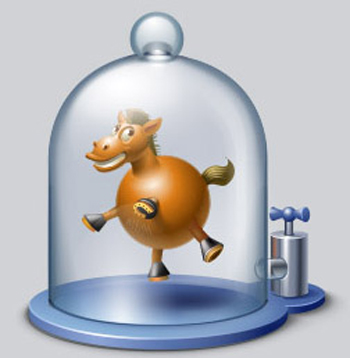
\includegraphics[height=.8\textheight]{Sphere_horse} %так вставляется картинка
	\end{center}
\end{frame} %конец слайда

\subsection{О сабже}
\begin{frame}{Высказывания о коне}
	\pause    % имитация анимации
	\begin{block}{Дарт Херохито}
 		"Так вот ты какой, северный олень!"
	\end{block}
	\pause
	\begin{block}{Кавалерия Новодворская}
 		"Сферический конь борозды не портит"
	\end{block}
	\pause
	\begin{block}{Русская женщина}
 		"Да я его на скаку!"
	\end{block}
\end{frame}

\section{Часть скучная}
\begin{frame}\frametitle{Пример перечислений и формул} 
	\begin{itemize}
		\item Раз
		\item Два
	\end{itemize}
	\begin{equation}
    	Русский_{низ}^{вверх} = \frac{всё}{работает^2\dots} = E = m c^2
	\end{equation}
\end{frame}

\begin{frame}\frametitle{Пример разбивания на столбцы}
 	\begin{columns}
 		\column{0.5\textwidth}
 			Содержимое левого столбца
 		\column{0.5\textwidth}
 			Содержимое правого столбца
 	\end{columns}
\end{frame}

\begin{frame}\frametitle{Жирный, курсивный текст, подчёркивание, ссылки}
	Если нужен жирный шрифт, то \textbf{это его пример}.

	А ещё можно \textit{побаловаться курсивом}. Или \emph{выспользоваться выделением текста}.

	Для особых случаев можно ещё и \underline{подчёркнутый текст} задействовать.

	А если вы знаете что такое капитель, то \textsc{можно ещё и так}. Почитать что такое капитель можно \href{https://ru.wikipedia.org/wiki/\%D0\%9A\%D0\%B0\%D0\%BF\%D0\%B8\%D1\%82\%D0\%B5\%D0\%BB\%D1\%8C_\%28\%D1\%88\%D1\%80\%D0\%B8\%D1\%84\%D1\%82\%29}{в статье на Википедии (ссылка)}.

	Кроме того, можно оформлять ссылки без текста, просто адрес ссылки \url{https://en.wikibooks.org/wiki/LaTeX}.
\end{frame}

\frame{\finalslide{Вопросы?}} %слайд вопросы?

\begin{frame}{Сферический список литературы в вакууме}
	\begin{thebibliography}{10}
	\beamertemplatebookbibitems
	\bibitem{LurkHorse}
		{\sc Lurkmore}, {\em \href{http://lurkmore.to/\%D0\%A1\%D1\%84\%D0\%B5\%D1\%80\%D0\%B8\%D1\%87\%D0\%B5\%D1\%81\%D0\%BA\%D0\%B8\%D0\%B9_\%D0\%BA\%D0\%BE\%D0\%BD\%D1\%8C_\%D0\%B2_\%D0\%B2\%D0\%B0\%D0\%BA\%D1\%83\%D1\%83\%D0\%BC\%D0\%B5}{Сферический конь в вакууме}}.
	\bibitem{AbsHorse}
		{\sc Абсурдопедия}, {\em \href{http://absurdopedia.wikia.com/wiki/\%D0\%A1\%D1\%84\%D0\%B5\%D1\%80\%D0\%B8\%D1\%87\%D0\%B5\%D1\%81\%D0\%BA\%D0\%B8\%D0\%B9_\%D0\%BA\%D0\%BE\%D0\%BD\%D1\%8C_\%D0\%B2_\%D0\%B2\%D0\%B0\%D0\%BA\%D1\%83\%D1\%83\%D0\%BC\%D0\%B5}{Сферический конь в вакууме}}.
	\bibitem{Horse}
		{\sc Муза}, {\em \url{http://ego-machine.blogspot.com/2010/03/latex-beamer.html}}.
	\end{thebibliography}
\end{frame}

\end{document}
